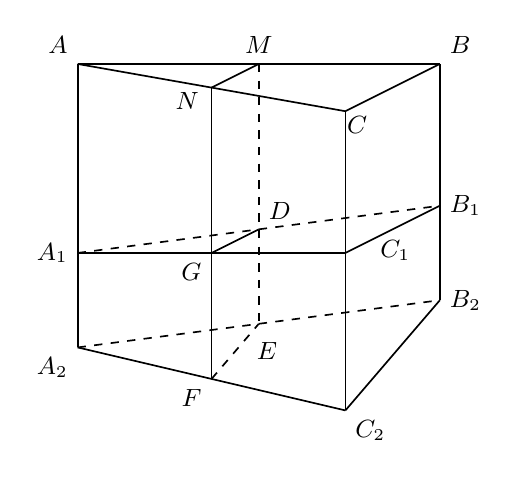
\begin{tikzpicture}[line width=.6pt, font=\small, >=stealth]
% schematic oblique prism; top z=4, mid z=2, bottom z=0
\coordinate (A) at (0,4);
\coordinate (M) at (2.3000000000,4.0000000000);
\coordinate (B) at (4.6,4);
\coordinate (N) at (1.7000000000,3.7000000000);
\coordinate (C) at (3.4000000000,3.4000000000);
\coordinate (A1) at (0,1.6);
\coordinate (G) at (1.7000000000,1.6000000000);
\coordinate (C1) at (3.4000000000,1.6000000000);
\coordinate (B1) at (4.6,2.2);
\coordinate (D) at (2.3000000000,1.9000000000);
\coordinate (A2) at (0,0.4);
\coordinate (F) at (1.7000000000,0.0000000000);
\coordinate (E) at (2.3000000000,0.7000000000);
\coordinate (B2) at (4.6,1.0);
\coordinate (C2) at (3.4000000000,-0.4000000000);
% top face
\draw (A)--(M)--(B);
\draw (A)--(N)--(C)--(B);
\draw (M)--(N);
% verticals
\draw (A)--(A1)--(A2);
\draw (B)--(B1)--(B2);
\draw (C)--(C1)--(C2);
\draw (N)--(G)--(F);
\draw[dashed] (M)--(D)--(E);
\draw[dashed] (F)--(E);
% middle and bottom
\draw (A1)--(G)--(C1);
\draw[dashed] (A1)--(B1);

\draw (C1)--(B1);

\draw[dashed] (A2)--(E)--(B2);
\draw (A2)--(F)--(C2);

\draw (G)--(D);
\node[above left] at (A) {$A$};
\node[above] at (M) {$M$};
\node[above right] at (B) {$B$};
\node[left,xshift=-1pt,yshift=-5pt] at (N) {$N$};
\node[right,xshift=-3pt,yshift=-5pt] at (C) {$C$};
\node[left] at (A1) {$A_{1}$};
\node[below left] at (G) {$G$};
\node[right,xshift=9pt,yshift=1pt] at (C1) {$C_{1}$};
\node[right] at (B1) {$B_{1}$};
\node[above right] at (D) {$D$};
\node[below left] at (A2) {$A_{2}$};
\node[below left] at (F) {$F$};
\node[below,xshift=3pt,yshift=-3pt] at (E) {$E$};
\node[right] at (B2) {$B_{2}$};
\node[below right] at (C2) {$C_{2}$};
\draw (B2)--(C2);
\end{tikzpicture}
